\documentclass[12pt]{article}

% Language setting
\usepackage[utf8]{inputenc}
\usepackage[bulgarian]{babel}

% --------------------- Packages  --------------------
% Use biblatex
\usepackage{biblatex}
\addbibresource{bibliography.bib}
% Table thickness
\usepackage{ctable}
% Equations: SI units
\usepackage{siunitx}
% Approximately equal
\usepackage{amssymb}
% degrees symbol
\usepackage{gensymb}
% warning box
\usepackage{pifont,mdframed}

\newenvironment{warning}
  {\par\begin{mdframed}[linewidth=2pt, linecolor=white]%
    \begin{list}{}{\leftmargin=1cm
                   \labelwidth=\leftmargin}\item[\Large\ding{43}]}
  {\end{list}\end{mdframed}\par}

% --------------------- Title  --------------------
\addbibresource{bibliography.bib}

\begin{document}

% Anfang der Titelseite________________________________________________________________________________
\begin{titlepage}
	\flushleft
% 	\begin{center}
	%{\scshape\Large Werkstoffe III \hspace{2.5cm} Laborbericht \hspace{2.5cm}HS 2022 \par}
	{\scshape\Large Протокол X \hspace{2cm} Механика - практикум\par}
	\vspace{5cm}
	{\huge\bfseries Теорема на Хюйгенс-Щайнер\par}
	\vspace{1cm}
	{\LARGE\bfseries Лабораторно упражнение №7\par}
	\vspace{5cm}
    % {\LARGE\bfseries Физически Факултет към Софийски Университет ``Св. Климент Охридски \par}
    {\LARGE\bfseries Виолета Кабаджова, \par}
%   {\LARGE\bfseries Group: X\par}
    {\large\bfseries ККТФ, фак. номер: 3PH0600026\par}
	\vspace{1cm}
	
	{\large Физически Факултет, 
	
	Софийски Университет "Св. Климент Охридски"
	
	15 ноември 2022 г.\par}
	
\end{titlepage}

\section{Теоритична част}\label{sec:theoretical-part}
Теоремата на Хюйгенс-Щайнер спомага за определянето на инерчния момент на тяло спрямо произволна ос, свеждайки задачата до измерване на инерчния момент на това тяло спрямо ос, успоредна на търсната и минаваща през центъра на масите му, и измерване на разстоянието между двете оси. Взаимовръзката им се изразява чрез формула \ref{eq:main-eq-theorem}, където $I$ е инечният момент на тяло с маса $m$ спрямо произволна ос Oz, $I_0$ - инерчният момент на тялото спрямо успоредна ос, минаваща през центъра на масите му, $l$ - разстоянието между тези две оси.

\begin{equation}\label{eq:main-eq-theorem}
    I = I_0 + ml^2
\end{equation}

Изследването на инерчния момент на тяло спрямо дадени оси може да се извърши посредством торзионно махало - твърдо тяло, което е закачено на нишка с еластични свойства при усукване, преминаваща през центъра на масите му. Периодът на едно торзионно махало се определя от формула \ref{eq:torsion-pendulum}, където $T$ е периодът на махалото, $I$ е инерчният момент спрямо оста около която трепти, а $D$ - дирекционният момент на нишката.  

\begin{equation}\label{eq:torsion-pendulum}
    T = 2\pi \sqrt{\frac{I}{D}}
\end{equation}

\begin{figure}
    \centering
    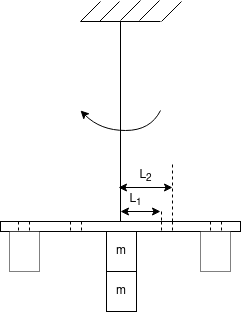
\includegraphics[width=0.4\textwidth]{images/parallel-axis-theorem.drawio.png}
    \caption{Схема на торзионно махало}
    \label{fig:setup}
\end{figure}

\section{Експериментална част}

\subsection{Експериментална установка}
На фиг. \ref{fig:setup} е указана схема на торзионно махало, което ще използваме в настоящия експеримент. То се състои от пръчка, върху която ще закрепим тела с маса $m$ на няколко разстояния от центъра на масите: $l_0 = 0$ cm, $l_1 = 23.8$ cm, $l_2 = 30.9$ cm, $l_3 = $ cm и $l_4 = 0$ cm. При $l_0 = 0$ cm, двете тела са окачени едно на друго.

Ще измерим инерчния момент на хомогенен диск, който в последствие ще заместим с пръчката. Разглеждането на хомогенен диск ни позволява да изследваме теоремата на Хюйгенс-Щайнер като съотношение между инерчните моменти на този диск и съответната система от пръчка и тела, използвайки формула \ref{eq:pendulum-inertia}, следваща от формули \ref{eq:torsion-pendulum} и \ref{eq:ratios-derivation}, като по този начин не се налага търсенето на дирекционния момент на системата. Чрез съпоставка на стойностите, получени от формули \ref{eq:main-eq-theorem} и \ref{eq:pendulum-inertia} за откриване на инерчния момент на тяло в рамките на техните грешки, ще докажем теоремата на Хюйгенс-Щайнер.

\begin{equation} \label{eq:ratios-derivation}
    \frac{T_c}{T_d} = \frac{2\pi \sqrt{\frac{I_c}{D}}}{2\pi \sqrt{\frac{I_d}{D}}} \Rightarrow \frac{I_c}{I_d} = \frac{T_c^2}{T_d^2}
\end{equation}

\begin{equation}\label{eq:pendulum-inertia}
    I_c = \frac{1}{2}MR^2\frac{T_c^2}{T_d^2}
\end{equation}

\subsection{Задача: Измерване на инерчния момент на хомогенния диск}
Инерчният момент на диск $I_d$ спрямо геометричната му ос може да бъде пресметната по формула \ref{eq:disk-inertia}, откъдето следва, че $I_d = (100.43 \pm 0.09)\cdot10^{-6}$ kg.m$^2$

\begin{equation}\label{eq:disk-inertia}
    I_d = \frac{1}{2}MR^2
\end{equation}

\subsection{Задача: Проверка на теоремата на Хюйгенс-Щайнер}
Валидността на теоремата ще потвърдим чрез сравняване на получените стойности за инерчния момент на системата от формули \ref{eq:main-eq-theorem} и \ref{eq:disk-inertia}, за които ще искаме да бъдат равни в рамките на абсолютните си грешки.

За по-голяма точност периода на диска изчисляваме чрез неколкократно измерване на времето за $N$ периода на диска, което сумарно време в последствие разделяме на $N$. 
% Получаваме $\bar{T} = 2.82 \pm 0.03$ s. 

За диска получаваме $\bar{T}_d = 2.82 \pm 0.03$ s, а за $\bar{T}_{c_{L1}} = 2.5128 \pm 0.01$ s,  $\bar{T}_{c_{L2}} = 2.91 \pm 0.01$ s,  $\bar{T}_{c_{L3}} = 4.13 \pm 0.01$ s,  $\bar{T}_{c_{L4}} = 4.62 \pm 0.01$ s.
Резултатите от пресмятанията представяме в таблица \ref{tbl:results}. Заключваме, че резултатите са верни в рамките на абсолютните си грешки, откъдето и валидираме теоремата на Хюйгенс-Щайнер.


\begin{table}[h]
\begin{center}
\begin{tabular}{|l|l|l|}\hline
L_i, [cm] & $I_c \cdot 10^{-6}$ по формула (\ref{eq:main-eq-theorem}) & $I_c \cdot 10^{-6}$ по формула (\ref{eq:pendulum-inertia}) \\ \hline
23.78 &79.82249 \pm 0.2 &79.82244 \pm 0.07\\ \hline
30.93 &107.1994 \pm 0.3 &107.1993 \pm 0.01\\ \hline
25.02 &216.1212 \pm 0.5 &216.1211 \pm 0.2\\ \hline
28.78 &270.3344 \pm 0.6 &270.3343 \pm 0.2\\ \hline
\end{tabular}
\caption{\label{tbl:results}Изчисляване на инерчния момент I_c  по два начина. [I_c] = kgm^2.}
\end{center}
\end{table}


\end{document}
